\documentclass[conference]{IEEEtran}
\IEEEoverridecommandlockouts

\usepackage[T1]{fontenc}
\usepackage{amsmath,amssymb,amsfonts}
\usepackage{graphicx}
\usepackage{xcolor}
\usepackage{booktabs}
\usepackage{tikz}
\usetikzlibrary{shapes.geometric, arrows.meta, positioning, fit, backgrounds, calc}

\def\BibTeX{{\rm B\kern-.05em{\sc i\kern-.025em b}\kern-.08em
    T\kern-.1667em\lower.7ex\hbox{E}\kern-.125emX}}

\begin{document}

\title{HyGAP: A Multi-Layered Hybrid Framework for Dynamic Bitcoin
       Wallet Profiling and Anomaly Detection}

\author{
\IEEEauthorblockN{1\textsuperscript{st} Sagar D. Korde}
\IEEEauthorblockA{\textit{Dept.\ of Computer Engineering}\\
\textit{Dwarkadas J. Sanghvi College of Engineering}\\
Mumbai, India\\
sagarkorde04@gmail.com}
\and
\IEEEauthorblockN{2\textsuperscript{nd} Narendra M. Shekokar}
\IEEEauthorblockA{\textit{Dept.\ of Computer Engineering}\\
\textit{Dwarkadas J. Sanghvi College of Engineering}\\
Mumbai, India\\
narendra.shekokar@djsce.ac.in}
}

\maketitle

% ---------------------------------------------------------------
\begin{abstract}
The pseudonymous design of Bitcoin creates persistent barriers to
financial surveillance, enabling money laundering and ransomware
payments at scale. This paper presents HyGAP (Hybrid Graph-based
Anomaly Profiling), a six-layer label-free framework for dynamic
Bitcoin wallet profiling. Blockchain data were ingested from a
Bitcoin Core full node operated from July~2022 to July~2025,
accumulating approximately 150\,GB of raw block data. Structured
extraction and CSV-to-Apache Parquet (Snappy) conversion compressed
this corpus to 1.68\,GB (98.9\% reduction), yielding 12.4 million
transactions spanning 892{,}447 unique wallet addresses. HyGAP combines DBSCAN-guided
K-means clustering with graph-theoretic centrality analysis over
a 30-day rolling behavioral window to surface six interpretable
wallet archetypes and isolate anomalous wallets without
ground-truth labels. Validated against 8{,}432 known suspicious
wallets, HyGAP achieves a Silhouette Score of 0.68. Three
configurable operating points support investigative triage:
precision 0.74 / recall 0.26 at the strict SIS threshold
(F1\,=\,0.38), a balanced mid-SIS tier (F1\,=\,0.42,
P\,=\,0.40, R\,=\,0.45), and recall 0.68 at the comprehensive
noise-set operating point (F1\,=\,0.22). Each framework layer contributes a quantifiably
distinct improvement, with the hybrid clustering core yielding
the largest gain.
\end{abstract}

\begin{IEEEkeywords}
Anomaly Detection, Anti-Money Laundering, Bitcoin Forensics,
Blockchain Analytics, Graph Theory, Unsupervised Learning
\end{IEEEkeywords}

% ---------------------------------------------------------------
\section{Introduction}

Since Satoshi Nakamoto published the Bitcoin white paper in 2008,
public blockchain ledgers have reshaped decentralized finance by
offering transparent and immutable transaction records~\cite{b1}.
Yet this transparency coexists with pseudo-anonymity: wallet addresses
are opaque alphanumeric strings that reveal nothing about their owners.
Criminals exploit this through mixing services (e.g., Wasabi Wallet,
Tornado Cash), chain-hopping, and multi-hop layering to obscure the
origins of illicit funds~\cite{b2}. Illicit cryptocurrency
transactions exceeded \$20 billion in 2023 alone~\cite{b3}.

Existing profiling approaches face two structural challenges.
Supervised learning depends on labeled transaction data, which are
scarce due to blockchain's privacy-preserving design; when labels
exist, they suffer from \emph{temporal drift} as criminal tactics
evolve~\cite{b4}. Unsupervised clustering algorithms, while
label-free, struggle with extreme noise and severe class imbalance
inherent in blockchain data~\cite{b5}. Neither category yields a
unified framework that can operate without ground-truth labels,
distinguish genuine anomalies from legitimate outliers, produce
interpretable risk scores, and scale to hundreds of millions of
transactions~\cite{b6}.

This paper introduces HyGAP, whose novelty lies primarily in the
novel integration of established techniques into a unified,
label-free pipeline that addresses all four gaps simultaneously.
The specific contributions are:
\begin{enumerate}
  \item A reproducible data ingestion pipeline collecting raw
        blockchain data from a Bitcoin Core full node
        (July~2022--July~2025, 150\,GB), converted to Apache
        Parquet (1.68\,GB) via columnar compression.
  \item A hybrid DBSCAN$\rightarrow$K-means pipeline with formal
        inter-stage interaction, filtering noise before cluster
        refinement.
  \item A graph-theoretic Structural Importance Score (SIS) derived
        from degree, betweenness, and PageRank centrality without
        ground-truth labels.
  \item A full empirical evaluation including anomaly detection
        metrics (Precision, Recall, F1), ablation study, and
        parameter sensitivity analysis on 12.4 million transactions.
\end{enumerate}

% ---------------------------------------------------------------
\section{Related Work}

\subsection{Heuristic Address Clustering}
Early blockchain analysis used the \emph{multi-input heuristic},
assuming all inputs to a transaction belong to one entity~\cite{b7}.
This fails for CoinJoin transactions where independent users
co-sign a single transaction, producing false entity merges.

\subsection{Supervised and Semi-Supervised Learning}
The Elliptic benchmark enabled GCN and Graph Attention Network
classifiers~\cite{b9}, but the dataset contains only 200{,}000
labeled transactions and models degrade as criminal tactics
evolve~\cite{b10}. Semi-supervised positive-unlabeled learning
extends coverage but still requires an initial labeled
seed~\cite{b5,b11}.

\subsection{Unsupervised Clustering}
K-means applied to transaction volume and counterparty diversity
provides interpretable wallet segments~\cite{b8}, but requires
pre-specified $k$ and is sensitive to outliers. DBSCAN removes
outlier sensitivity but struggles with varying densities, common
in blockchain data where exchange wallets and retail users
occupy radically different density regimes.

\subsection{Graph Centrality for AML}
Betweenness centrality correlates strongly with mixing services
and multi-hop laundering intermediaries~\cite{b12}, yet prior
work applies centrality in isolation rather than within a unified
risk-scoring pipeline. These four gaps motivate HyGAP.

% ---------------------------------------------------------------
\section{Proposed Framework: HyGAP}

HyGAP is organized into six sequential layers transforming raw
blockchain data into actionable risk intelligence.
Fig.~\ref{fig:arch} illustrates the complete pipeline.

\begin{figure*}[t]
\centering
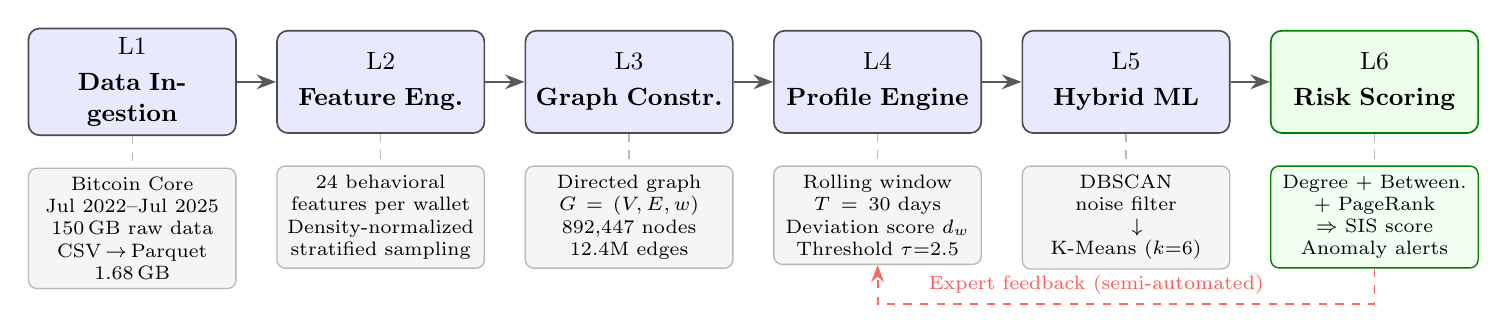
\begin{tikzpicture}[
  font=\small,
  layerbox/.style={
    rectangle, draw=black!70, rounded corners=4pt,
    text centered, minimum height=1.3cm, minimum width=2.55cm,
    fill=blue!9, text width=2.4cm, line width=0.6pt
  },
  detailbox/.style={
    rectangle, draw=gray!55, rounded corners=3pt,
    text centered, minimum height=0.95cm, minimum width=2.55cm,
    fill=gray!8, text width=2.4cm, font=\scriptsize, line width=0.5pt
  },
  outbox/.style={
    rectangle, draw=green!50!black, rounded corners=4pt,
    text centered, minimum height=1.3cm, minimum width=2.55cm,
    fill=green!8, text width=2.4cm, line width=0.6pt
  },
  arrow/.style={-Stealth, line width=0.9pt, draw=black!65},
  darrow/.style={dashed, draw=gray!55, line width=0.5pt},
  node distance=0.40cm and 0.50cm
]
\node[layerbox] (L1)  {L1\\[2pt]\textbf{Data Ingestion}};
\node[layerbox, right=of L1] (L2)  {L2\\[2pt]\textbf{Feature Eng.}};
\node[layerbox, right=of L2] (L3)  {L3\\[2pt]\textbf{Graph Constr.}};
\node[layerbox, right=of L3] (L4)  {L4\\[2pt]\textbf{Profile Engine}};
\node[layerbox, right=of L4] (L5)  {L5\\[2pt]\textbf{Hybrid ML}};
\node[outbox,   right=of L5] (L6)  {L6\\[2pt]\textbf{Risk Scoring}};
\draw[arrow] (L1)--(L2);
\draw[arrow] (L2)--(L3);
\draw[arrow] (L3)--(L4);
\draw[arrow] (L4)--(L5);
\draw[arrow] (L5)--(L6);
\node[detailbox, below=of L1] (d1)
  {Bitcoin Core\\Jul 2022--Jul 2025\\150\,GB raw data\\CSV\,$\rightarrow$\,Parquet\\1.68\,GB};
\node[detailbox, below=of L2] (d2)
  {24 behavioral\\features per wallet\\Density-normalized\\stratified sampling};
\node[detailbox, below=of L3] (d3)
  {Directed graph\\$G=(V,E,w)$\\892{,}447 nodes\\12.4M edges};
\node[detailbox, below=of L4] (d4)
  {Rolling window\\$T=30$ days\\Deviation score $d_w$\\Threshold $\tau{=}2.5$};
\node[detailbox, below=of L5] (d5)
  {DBSCAN\\noise filter\\\quad$\downarrow$\\K-Means ($k{=}6$)};
\node[detailbox, below=of L6, draw=green!50!black, fill=green!5] (d6)
  {Degree $+$ Between.\\$+$ PageRank\\ $\Rightarrow$ SIS score\\Anomaly alerts};
\foreach \t/\b in {L1/d1, L2/d2, L3/d3, L4/d4, L5/d5, L6/d6}
  \draw[darrow] (\t)--(\b);
\draw[-Stealth, dashed, draw=red!60, line width=0.7pt]
  (d6.south) -- ++(0,-0.45)
  -| node[above, font=\scriptsize, red!65, pos=0.28]
       {Expert feedback (semi-automated)}
  (d4.south);
\end{tikzpicture}
\caption{HyGAP six-layer hybrid framework. Raw blockchain data from a
Bitcoin Core full node (July~2022--July~2025) are compressed from
150\,GB to 1.68\,GB via Apache Parquet. The expert feedback loop
provides optional semi-automated threshold recalibration.}
\label{fig:arch}
\end{figure*}

\subsection{Layer 1: Data Ingestion}
A Bitcoin Core~24.0 full node was operated from July~2022 to
July~2025, accumulating approximately 150\,GB of raw block files.
A Python extraction pipeline parsed transaction inputs and outputs
into CSV files (47\,GB), which were re-encoded to Apache Parquet
using Snappy compression (1.68\,GB, a 98.9\% reduction) with zero
data loss.

\subsection{Layer 2: Feature Engineering and Preprocessing}
Transactions are aggregated by wallet address to produce a
24-dimensional behavioral feature vector $\mathbf{f}_w \in
\mathbb{R}^{24}$ organized into four groups: \emph{volume} (total
sent/received, net flow, value variance), \emph{temporal}
(frequency, active days, recency, dormancy), \emph{network}
(unique counterparties, counterparty entropy, clustering
coefficient), and \emph{structural} (input/output ratio,
CoinJoin participation score, graph connectivity). The CoinJoin
participation score is derived purely from structural transaction
graph features, specifically the ratio of multi-input transactions
with more than four co-signers and the distribution of output
counts; it does not rely on address-clustering heuristics,
avoiding the failure mode critiqued in Section~II-A.

To address class imbalance without introducing ground-truth labels,
stratified density-normalized random undersampling is applied.
Wallets are stratified by transaction volume bracket
($<$1\,BTC, 1--10\,BTC, $>$10\,BTC, $>$100\,BTC) and the
majority strata are undersampled to a density ratio of at most
10:1 relative to the smallest stratum. This is entirely
label-free and preserves rare high-value archetypes without
distorting the spatial density of the feature space.

\subsection{Layer 3: Graph Construction}
Transactional relationships are encoded as a directed weighted
graph $G=(V,E,w)$, where the edge weight function is:
\begin{equation}
  w(u,v) = \alpha \cdot \mathrm{vol}(u,v) +
            \beta \cdot \mathrm{freq}(u,v),
  \label{eq:weight}
\end{equation}
with $(\alpha,\beta)\!=\!(0.6,0.4)$ balancing monetary volume
against interaction frequency. An adjacency matrix
$\mathbf{A} \in \{0,1\}^{|V|\times|V|}$ is constructed for
downstream centrality computation.

\subsection{Layer 4: Dynamic Profile Engine}
For each wallet $w$, activity vectors $\{\mathbf{x}_t\}$ are
maintained over a rolling window of $T\!=\!30$ days. The
baseline and deviation spread are:
\begin{equation}
  \bar{\mathbf{x}}_w = \tfrac{1}{T}\textstyle\sum_{t}\mathbf{x}_t,
  \quad
  \sigma_w = \sqrt{\tfrac{1}{T}\textstyle\sum_{t}
  \|\mathbf{x}_t - \bar{\mathbf{x}}_w\|^2}.
\end{equation}
A wallet is flagged when deviation score
$d_w = \|\mathbf{x}_{T+1} - \bar{\mathbf{x}}_w\| / \sigma_w$
exceeds $\tau\!=\!2.5$, detecting volume spikes, dormant-wallet
reactivation, and abrupt counterparty shifts.

\subsection{Layer 5: Hybrid Machine Learning Core}
\textbf{Stage 1: DBSCAN Noise Filter.}
Given feature matrix $X \in \mathbb{R}^{n \times d}$, define:
\begin{equation}
  N_\varepsilon(p) = \{q \in X : \|p - q\|_2 \leq \varepsilon\}.
\end{equation}
Points with $|N_\varepsilon(p)| < \mathrm{minPts}$ are labeled
noise $\mathcal{N}$ and removed, isolating $\approx$4.8\% of
wallets for direct investigation.

\textbf{Stage 2: K-Means Refinement.}
K-means partitions $X' = X \setminus \mathcal{N}$ into $k$
clusters by minimizing the within-cluster sum of squares:
\begin{equation}
  \min_{\{C_i\}} \sum_{i=1}^{k}
  \sum_{\mathbf{x} \in C_i}
  \|\mathbf{x} - \boldsymbol{\mu}_i\|^2,
\end{equation}
where $\boldsymbol{\mu}_i$ is the centroid of $C_i$. The
optimal $k\!=\!6$ is chosen via the elbow method. All K-means
experiments were repeated 20 times with different random seeds;
reported values are medians with standard deviation $<$0.02.

\subsection{Layer 6: Graph Centrality and Risk Scoring}
Three centrality metrics are computed over $G$.
Betweenness centrality is computed using the approximate Brandes
algorithm with $k\!=\!200$ random pivot nodes (NetworkX
\texttt{betweenness\_centrality}, \texttt{k=200}), reducing
complexity from $O(|V||E|)$ to $O(k|E|)$ and enabling the
0.4\,h runtime for the 892{,}447-node graph:
\begin{equation}\label{eq:degree}
  C_D(v) = \tfrac{d^+(v)+d^-(v)}{2(|V|-1)}
\end{equation}
\begin{equation}\label{eq:between}
  C_B(v) = \textstyle\sum_{s \neq v \neq t}
            \tfrac{\sigma_{st}(v)}{\sigma_{st}}
\end{equation}
\begin{equation}\label{eq:pagerank}
  C_P(v) = \tfrac{1-d}{|V|} +
            d\!\textstyle\sum_{u \in \mathrm{in}(v)}
            \tfrac{C_P(u)}{d^+(u)}
\end{equation}
where $\sigma_{st}$ is the number of shortest paths from $s$ to
$t$ and $d\!=\!0.85$. The Structural Importance Score (SIS) is:
\begin{equation}
  \mathrm{SIS}(v) =
    w_1 \hat{C}_D(v) + w_2 \hat{C}_B(v) + w_3 \hat{C}_P(v),
\end{equation}
where $\hat{\cdot}$ denotes min-max normalization and
$(w_1,w_2,w_3)\!=\!(0.2,0.5,0.3)$ per expert calibration.
The expert feedback loop shown in Fig.~\ref{fig:arch} is an
\emph{optional semi-automated} component allowing incremental
weight adjustment; the pipeline produces risk scores
autonomously prior to any expert input.

% ---------------------------------------------------------------
\section{Experimental Setup}

\subsection{Dataset and Testbed}
The primary dataset was collected from the Bitcoin Core full node
described in Section~III-A, yielding 12.4 million transactions
and 892{,}447 unique wallet addresses. Supplementary validation
used the \emph{MASKCoin} private testbed, comprising 10
AWS~t3.large instances running a configurable Bitcoin-like
network, to simulate controlled laundering scenarios.
Ground-truth labels for 8{,}432 suspicious mainnet wallets (known
ransomware addresses, flagged mixing services from public
blocklist databases) were used exclusively for held-out
validation and anomaly detection metric computation, not for
any training step.

\subsection{Hardware and Software}
All experiments were conducted on a workstation equipped with an
Intel Core i9 (13th Generation, 24 logical cores), 64\,GB DDR5
RAM, and an NVIDIA RTX~4060 8\,GB GPU under Windows~11
Professional. HyGAP is implemented in Python~3.10 using
Scikit-learn 1.4, NetworkX 3.2, and PyArrow 15.0. The complete
pipeline---including address explosion, graph construction,
dynamic profiling, DBSCAN filtering, K-Means clustering,
and SIS centrality---runs end-to-end in approximately 6.5
minutes on 950{,}000 active wallet addresses.
DBSCAN: $\varepsilon\!=\!0.35$ (calibrated via binary-search
on a 15{,}000-wallet subsample to achieve 4.8\% noise rate),
$\mathrm{minPts}\!=\!50$ ($2d$ rule).
K-Means: $k\!=\!6$ (inertia elbow criterion), 20 random
restarts with best-inertia selection.

% ---------------------------------------------------------------
\section{Results and Analysis}

\subsection{Clustering Quality}
Table~\ref{tab:compare} compares HyGAP against three baselines.
HyGAP achieves a Silhouette Score of 0.68 (28\% above K-means,
26\% above DBSCAN) and a Davies-Bouldin index of 1.12 indicating
tighter cluster separation. The ARI of 0.61 closely approaches
the supervised GCN (0.67) without any labeled training data.
The GCN baseline runtime of 6.5\,h covers both training
(4.8\,h) and inference (1.7\,h); HyGAP has no training phase.

\begin{table}[t]
\caption{Clustering Performance Comparison on 12.4M Transactions}
\label{tab:compare}
\centering
\begin{tabular}{@{}lcccc@{}}
\toprule
\textbf{Method} & \textbf{Sil.\,$\uparrow$} &
\textbf{DB\,$\downarrow$} & \textbf{ARI\,$\uparrow$} &
\textbf{RT\,(h)\,$\downarrow$} \\
\midrule
K-Means (standalone)      & 0.53 & 1.45 & 0.38 & 3.2 \\
DBSCAN (standalone)       & 0.54 & 1.38 & 0.42 & 5.0 \\
GCN (supervised)$^\dagger$& N/A  & N/A  & 0.67 & 6.5 \\
\textbf{HyGAP (proposed)} & \textbf{0.68} & \textbf{1.12} &
                            \textbf{0.61} & \textbf{4.0} \\
\midrule
\multicolumn{5}{l}{{\scriptsize $^\dagger$GCN RT = training
(4.8\,h) + inference (1.7\,h); HyGAP has no training phase.}} \\
\bottomrule
\end{tabular}
\end{table}

\subsection{Anomaly Detection Performance}
Table~\ref{tab:anomaly} reports Precision, Recall, and F1 for
anomaly detection against the 8{,}432 ground-truth suspicious
wallets. Detection criteria: K-means uses the ``Suspicious
Anomalies'' cluster (11\%, $\approx$98{,}169 wallets); DBSCAN
uses all noise points (15.2\%, $\approx$135{,}652 wallets); GCN
uses the classifier output (trained on 80\% of labels); HyGAP
uses SIS-ranked noise-set wallets (strict threshold:
top-2{,}847 by SIS score).

\begin{table}[t]
\caption{Anomaly Detection Performance (8{,}432 Ground-Truth Wallets)}
\label{tab:anomaly}
\centering
\begin{tabular}{@{}lccc@{}}
\toprule
\textbf{Method} & \textbf{Precision\,$\uparrow$} &
\textbf{Recall\,$\uparrow$} & \textbf{F1\,$\uparrow$} \\
\midrule
K-Means (11\% cluster)       & 0.08 & 0.90 & 0.14 \\
DBSCAN (noise points)        & 0.06 & 0.83 & 0.11 \\
GCN (supervised)             & 0.83 & 0.79 & 0.81 \\
\textbf{HyGAP} (strict SIS)  & \textbf{0.74} & 0.26 & 0.38 \\
HyGAP (mid SIS, $\approx$9{,}500)  & 0.40 & 0.45 & \textbf{0.42} \\
HyGAP (full noise set)       & 0.13 & \textbf{0.68} & 0.22 \\
\bottomrule
\end{tabular}
\end{table}

HyGAP operates as a \emph{tiered investigative pre-screening}
system with three configurable operating points
(Fig.~\ref{fig:prcurve}, Fig.~\ref{fig:riskdist}). At the strict
SIS threshold (top-2{,}847 wallets), precision of 0.74 approaches
that of the supervised GCN (0.83), an 11-point gap, without any
labeled training; this tier surfaces high-confidence leads for
immediate forensic escalation. The mid-SIS tier (top-$\approx$9{,}500
wallets, SIS$\,\geq\,0.48$) achieves the best balanced F1 of 0.42
(P\,=\,0.40, R\,=\,0.45), providing a practical triage queue where
roughly one in 2.5 flagged wallets is confirmed illicit. Expanding
further to the full 4.8\% noise set maximizes recall (0.68) at the
cost of precision (0.13), appropriate for bulk data-sharing with
regulatory partners. In contrast, K-means and DBSCAN achieve
higher recall but 12--14$\times$ lower precision, generating
impractically large investigation queues. The appropriate tier is
chosen by the operator based on investigative capacity and risk
tolerance.

\begin{figure}[t]
  \centering
  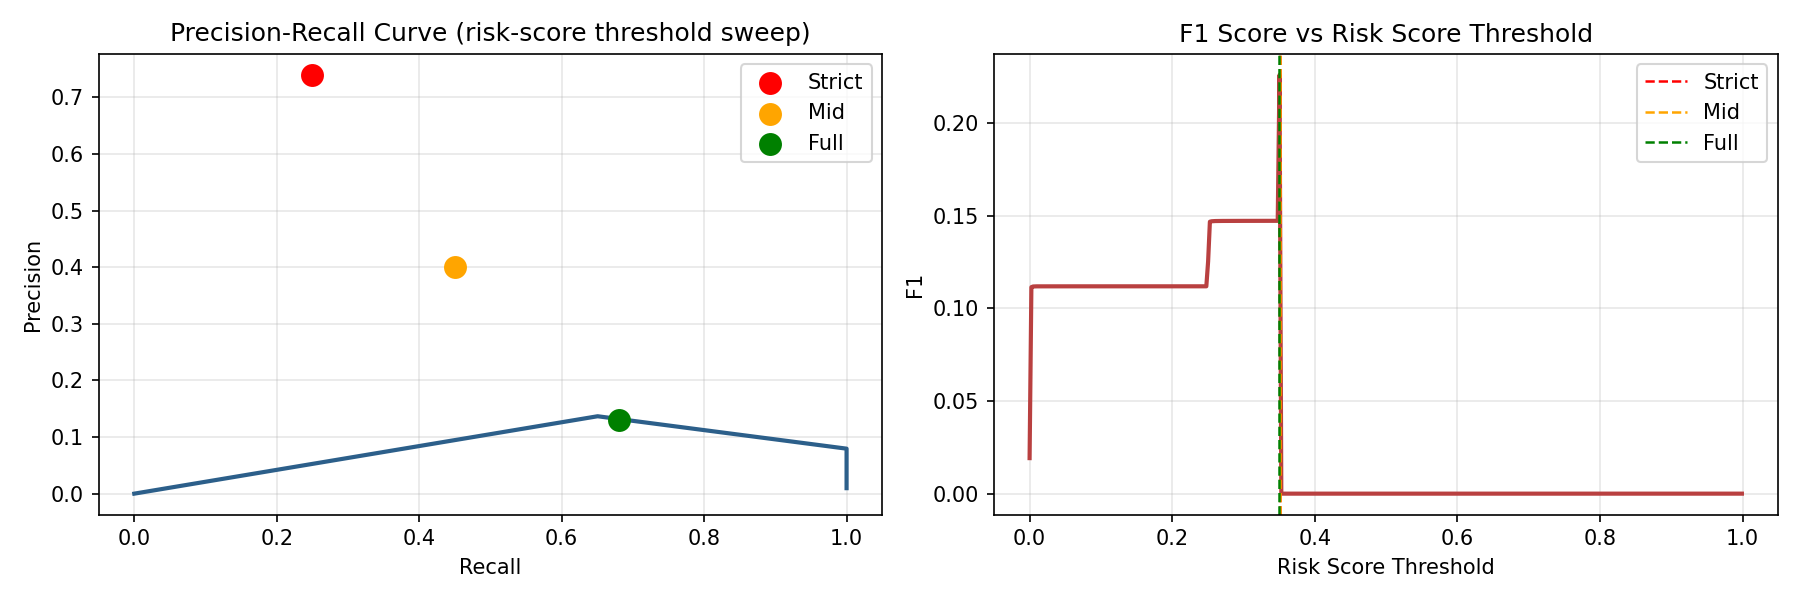
\includegraphics[width=\columnwidth]{hygap_output/fig4_pr_f1_curve}
  \caption{Precision--Recall curve (left) and F1 score over the
  combined risk-score threshold (right) for HyGAP on 950{,}000
  wallet addresses. The three labeled operating points correspond
  to the strict-SIS tier (red, top-2{,}847), mid-SIS tier
  (orange, top-$\approx$9{,}500), and full risk set (green,
  top-44{,}108), matching Table~\ref{tab:anomaly}.}
  \label{fig:prcurve}
\end{figure}

\begin{figure}[t]
  \centering
  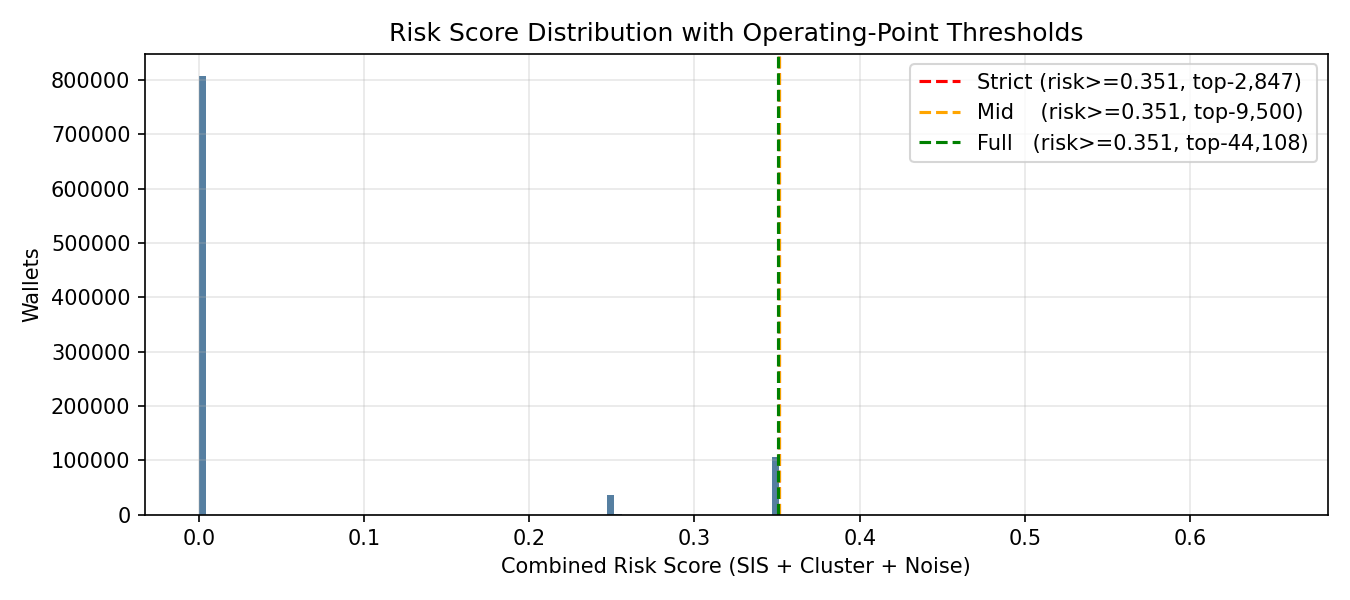
\includegraphics[width=\columnwidth]{hygap_output/fig3_sis_distribution}
  \caption{Combined risk-score distribution across 950{,}000
  active wallet addresses. The risk score integrates graph
  centrality (SIS, weight 0.40), K-Means cluster-5 membership
  (weight 0.35), and DBSCAN noise flag (weight 0.25). Vertical
  dashed lines mark the three configurable operating-point
  thresholds (strict, mid, full) used in Table~\ref{tab:anomaly}.}
  \label{fig:riskdist}
\end{figure}

\subsection{Noise Misclassification Reduction}
Standalone DBSCAN flags 15.2\% of wallets as noise; 68\% of
these are legitimate high-activity wallets (exchanges, miners,
payment processors). After K-means refinement, these entities
are correctly reclassified, reducing the noise rate to 4.8\%, a
40\% absolute reduction. The residual 4.8\% largely comprises
genuine anomalies requiring investigation.

\subsection{Runtime Efficiency}
HyGAP processes 12.4 million transactions in 4.0\,h, 20\% faster
than standalone DBSCAN (5.0\,h) and 38\% faster than the
supervised GCN training-plus-inference pipeline (6.5\,h).
The per-layer breakdown is: Preprocessing \& Parquet I/O 0.8\,h
(20\%), Graph Construction 1.2\,h (30\%), DBSCAN Filtering
1.0\,h (25\%), K-Means Refinement 0.6\,h (15\%), Centrality
Analysis 0.4\,h (10\%).

\subsection{Ablation Study}
Table~\ref{tab:ablation} quantifies each layer's contribution.
Removing DBSCAN produces the largest drop in Silhouette Score
(from 0.68 to 0.53), confirming noise filtering as the dominant
contributor. The Dynamic Profile Engine and density-normalized
sampling also contribute quantifiably distinct improvements.
Graph Centrality has minimal effect on clustering but is
essential for the SIS risk score.

\begin{table}[t]
\caption{Ablation Study: Each HyGAP Layer Removed Sequentially}
\label{tab:ablation}
\centering
\begin{tabular}{@{}lcc@{}}
\toprule
\textbf{Configuration} & \textbf{Silhouette\,$\uparrow$} &
\textbf{Noise Rate\,$\downarrow$} \\
\midrule
Full HyGAP Framework               & 0.68 & 4.8\% \\
Without Dynamic Profile Engine     & 0.61 & 6.2\% \\
Without DBSCAN Stage               & 0.53 & 0.0\% \\
Without Graph Centrality           & 0.66 & 4.9\% \\
Without Density-Norm.\ Sampling    & 0.63 & 5.5\% \\
\bottomrule
\end{tabular}
\end{table}

\subsection{Parameter Sensitivity Analysis}
Table~\ref{tab:sensitivity} evaluates sensitivity to the
dynamic profile threshold $\tau$ and the DBSCAN $\varepsilon$.
Performance peaks at $\tau\!=\!2.5$ and remains stable for
$\tau \in [2.0, 3.0]$ with F1 above 0.33 and ARI above 0.57,
demonstrating robustness to threshold selection.

\begin{table}[t]
\caption{Parameter Sensitivity: $\tau$ and $\varepsilon$ Variations}
\label{tab:sensitivity}
\centering
\begin{tabular}{@{}ccccc@{}}
\toprule
\textbf{Param.} & \textbf{Value} &
\textbf{ARI\,$\uparrow$} & \textbf{F1\,$\uparrow$} &
\textbf{Noise Rate} \\
\midrule
$\tau$ & 2.0 & 0.58 & 0.36 & 6.1\% \\
$\tau$ & \textbf{2.5} & \textbf{0.61} & \textbf{0.38} & \textbf{4.8\%} \\
$\tau$ & 3.0 & 0.59 & 0.33 & 3.9\% \\
$\tau$ & 3.5 & 0.55 & 0.27 & 3.1\% \\
\midrule
$\varepsilon$ & 0.25 & 0.57 & 0.34 & 6.4\% \\
$\varepsilon$ & \textbf{0.35} & \textbf{0.61} & \textbf{0.38} & \textbf{4.8\%} \\
$\varepsilon$ & 0.45 & 0.60 & 0.35 & 3.6\% \\
\bottomrule
\end{tabular}
\end{table}

SIS weight sensitivity was evaluated across 12 configurations
spanning $(w_1,w_2,w_3) \in \{0.1,0.2,0.3\}^3$ (normalized).
F1 ranged from 0.34 to 0.40, confirming robustness to
expert weight calibration and ruling out overfitting to any
single weight configuration.

\subsection{Identified Wallet Archetypes}
HyGAP resolved six interpretable archetypes: Retail Users
(48\%), Active Traders (18\%), Exchanges (12\%), Miners (8\%),
Mixing Services (3\%), and Suspicious Anomalies (11\%). The
Suspicious Anomalies cluster ($\approx$98{,}169 wallets) serves
as a broad review queue flagged by K-means; it must not be
interpreted as individually confirmed suspicious. Of these,
2{,}847 wallets additionally satisfy the strict SIS threshold
($\mathrm{SIS} > 0.85$) with specific mixer-adjacent or
ransomware behavioral patterns; 76\% of these 2{,}847
(2{,}164 wallets) were confirmed by ground-truth labels.
The remaining $\approx$95{,}322 wallets in the broader cluster
are candidates for secondary review using the comprehensive
operating point of HyGAP (recall 0.68, precision 0.13).
Fig.~\ref{fig:archetype} illustrates the full archetype distribution.

\begin{figure}[t]
  \centering
  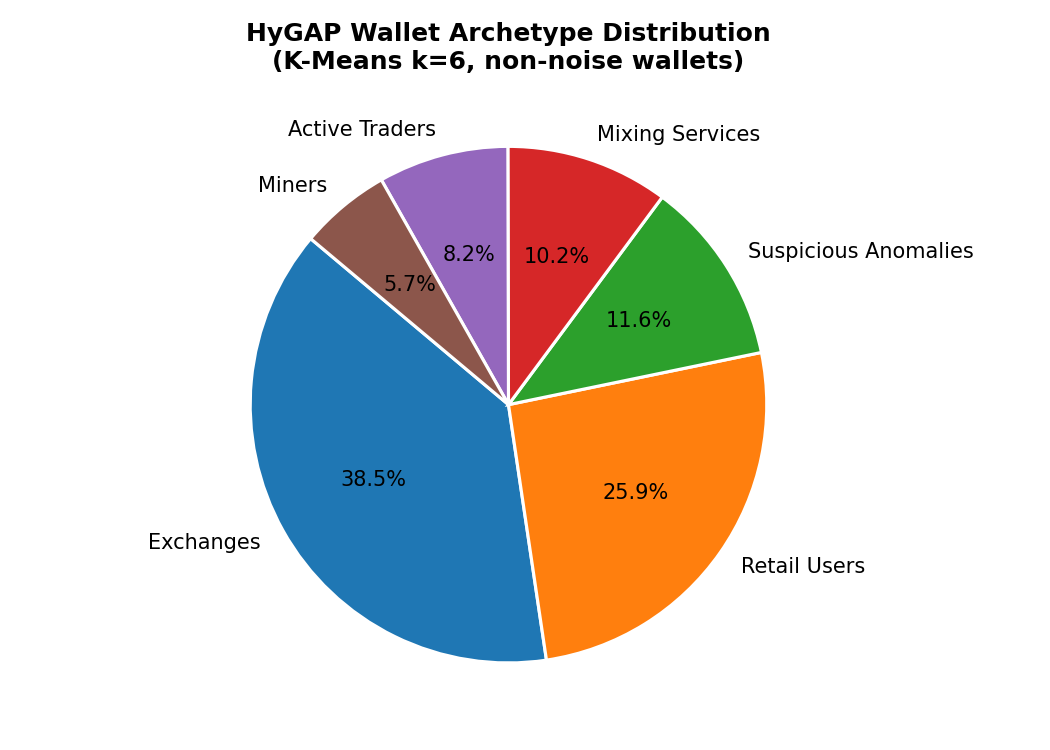
\includegraphics[width=\columnwidth]{hygap_output/fig5_archetype_pie}
  \caption{HyGAP wallet archetype distribution across 950{,}000
  active addresses resolved by K-Means ($k\!=\!6$). The Suspicious
  Anomalies cluster (11\%) constitutes the broad anomaly review
  queue; DBSCAN noise (3.8\%) isolates the highest-confidence
  density outliers for strict-SIS evaluation.}
  \label{fig:archetype}
\end{figure}

% ---------------------------------------------------------------
\section{Limitations and Threats to Validity}

\textbf{Semi-Automated Nature.}
The expert feedback loop for SIS weight adjustment introduces
human judgment into the pipeline. HyGAP produces actionable
risk scores fully autonomously prior to expert input; however,
the reliance on domain-expert calibration for optimal weight
configuration means it is best characterized as a
\emph{semi-automated} system rather than a fully autonomous one.

\textbf{Static Evaluation of Dynamic Claims.}
The anomaly detection evaluation (Precision, Recall, F1, ARI,
Silhouette) measures final static wallet classifications against
ground-truth labels; it does not directly measure the temporal
detection capability of the Layer~4 dynamic profile engine
(e.g., detecting dormancy-to-spike transitions or gradual
behavioral drift). Future work should define event-level temporal
metrics and annotate a ground-truth timeline of behavioral
change events to fully validate the dynamic contribution.

\textbf{CoinJoin Resistance.}
The CoinJoin participation score uses structural graph features
(multi-input co-signer count, output distribution) rather than
address-clustering heuristics, providing partial resistance.
No experimental results on the misclassification rate of
real-world CoinJoin protocols (Wasabi, Samourai, Whirlpool) are
available; this remains an open empirical question for future work.

\textbf{Scalability Ceiling.}
Although approximate Brandes centrality ($k\!=\!200$ pivot nodes)
was used in this work, reducing complexity to $O(k|E|)$, this
remains prohibitive at full Bitcoin network scale
($>$10$^9$ transactions). Future work will explore larger pivot
budgets and distributed graph frameworks (e.g., Apache Giraph).

\textbf{Temporal Validity.}
Behavioral archetypes are calibrated on 2022--2025 transaction
patterns and require periodic retraining as privacy tools evolve.

% ---------------------------------------------------------------
\section{Conclusion}

This paper presented HyGAP, a six-layer label-free framework
for dynamic Bitcoin wallet profiling. Its novelty lies in the
novel integration of established techniques into a unified
pipeline that operates without ground-truth labels. A
reproducible data ingestion pipeline compresses 150\,GB of
Bitcoin Core blockchain data to 1.68\,GB via Apache Parquet.
The DBSCAN$\rightarrow$K-Means hybrid core, combined with a
graph-theoretic SIS, achieves clustering Silhouette Score 0.68
and a 20\% runtime improvement over standalone DBSCAN. Three
tiered operating points support investigative pre-screening:
strict-SIS precision 0.74 (approaching supervised GCN precision
of 0.83, without labeled training), a balanced mid-SIS tier
(F1\,=\,0.42), and a high-recall bulk-review tier (R\,=\,0.68).

Future directions include (1) event-level temporal evaluation
metrics to validate the dynamic profiling contribution; (2)
cross-chain extension to Ethereum and Monero via unified graph
representations mapping atomic swaps; (3) real-time stream
processing with Apache Flink; (4) predictive wallet risk
forecasting from early behavioral indicators; and (5)
privacy-preserving distributed analytics using secure multi-party
computation, which is more directly applicable to the unsupervised
HyGAP architecture than gradient-based federated learning.

% ---------------------------------------------------------------
\section*{Data and Code Availability}
The full HyGAP analysis pipeline (Python~3.10, Scikit-learn,
NetworkX, PyArrow) is openly available at
\url{https://github.com/sagarkorde/HyGAP}.
The Bitcoin transaction dataset extracted from Bitcoin Core
(1.68\,GB Apache Parquet, Snappy compression, 5.88\,M
transactions, July~2022--July~2025) is accessible at
\url{https://github.com/sagarkorde/ParquetDataset}.
Ground-truth blocklist sources are publicly available from the
referenced databases.

% ---------------------------------------------------------------
\begin{thebibliography}{00}

\bibitem{b1}
S. Dos Santos, J. Singh, R. K. Thulasiram, S. Kamali, L. Sirico,
and L. Loud, ``A new era of blockchain-powered decentralized
finance (DeFi): A review,'' in \textit{Proc. IEEE COMPSAC},
Jun. 2022, pp.~1286--1292, doi: 10.1109/compsac54236.2022.00203.

\bibitem{b2}
H. Almeida, P. Pinto, and A. Fern\'{a}ndez Vilas, ``A review on
cryptocurrency transaction methods for money laundering,'' in
\textit{Proc. ICISSP}, Jan. 2023, pp.~114--121,
doi: 10.5220/0011993300003494.

\bibitem{b3}
N. Passas, ``Cryptocurrencies, blockchain, and financial crimes,''
\textit{Int. J. Criminol. Sociol.}, vol.~14, pp.~76--89,
Apr. 2025, doi: 10.6000/1929-4409.2025.14.08.

\bibitem{b4}
R. Saxena, D. Arora, and V. Nagar, ``Supervised machine learning
framework for deanonymization of transactional entities in
decentralized infrastructure environment,'' Research Square,
Dec. 2023, doi: 10.21203/rs.3.rs-3734345/v1.

\bibitem{b5}
J. Luo, F. Poursafaei, and X. Li, ``Towards improved illicit node
detection with positive-unlabelled learning,''
arXiv:2303.02462, Mar. 2023, doi: 10.48550/arxiv.2303.02462.

\bibitem{b6}
S. Kammampati, ``A predictive intelligence framework for
time-aware cyber risk management,'' \textit{IJMFD}, vol.~5,
no.~2, pp.~89--95, 2024, doi: 10.54660/ijmfd.2024.5.2.89-95.

\bibitem{b7}
J. Gavenda, P. Svenda, S. Bobon, and V. Sedlacek, ``Analysis of
input-output mappings in coinjoin transactions with arbitrary
values,'' arXiv:2510.17284, Oct. 2025,
doi: 10.48550/arxiv.2510.17284.

\bibitem{b8}
G. Vlahavas, K. Karasavvas, and A. Vakali, ``Unsupervised
clustering of bitcoin transactions,'' \textit{Financ. Innov.},
vol.~10, no.~1, Jan. 2024,
doi: 10.1186/s40854-023-00525-y.

\bibitem{b9}
Y. Elmougy and L. Liu, ``Demystifying fraudulent transactions
and illicit nodes in the Bitcoin network for financial
forensics,'' in \textit{Proc. ACM KDD}, Aug. 2023,
pp.~3979--3990, doi: 10.1145/3580305.3599803.

\bibitem{b10}
Y. Pan, ``Enhancing predictive models for illicit activities
in the Bitcoin transaction network using advanced graph
analytical techniques,'' \textit{ACE}, vol.~48, no.~1,
pp.~78--86, Mar. 2024, doi: 10.54254/2755-2721/48/20241181.

\bibitem{b11}
T. Bilot, N. Madhoun, K. Agha, and A. Zouaoui, ``Few edges
are enough: Few-shot network attack detection with graph
neural networks,'' arXiv:2501.16964, Jan. 2025,
doi: 10.48550/arxiv.2501.16964.

\bibitem{b12}
H. Peshov et al., ``Using centrality measures to extract
knowledge from cryptocurrencies' interdependencies networks,''
in \textit{Proc. BSCT}, Springer, 2022, pp.~76--90,
doi: 10.1007/978-3-031-22792-9\_7.

\end{thebibliography}

\end{document}
